\section{Turingmaschinen}
\subsection{Motivation}
\begin{frame}
	\frametitle{Motivation}
  \begin{block}{Wozu?}
    Wir wollen ein Konstrukt mit dem wir beweisen können, das Dinge berechenbar sind. (und wenn ja, wie lange wir dafür brauchen)
    Also wollen wir etwas konstruieren das \emph{alle} Algorithmen ausführen kann.
  \end{block}
  \begin{block}{Wie?}
    Wir formalisieren alle Handlungen die ein \emph{Mathematiker} ausführen kann:
    \begin{itemize}
      \item etwas von einem Blatt Papier lesen
      \item etwas auf ein Blatt Papier schreiben
      \item sich endliche viele Dinge merken
    \end{itemize}
  \end{block}
\end{frame}

\subsection{Definition}
\begin{frame}
	\frametitle{Partiellen Funktionen}
  \begin{definition}
	Eine \emph{partielle Funktion} $f: M_1 \dashrightarrow M_2$ ist rechtseindeutig aber nicht notwendigerweise linkstotal.\\
  \end{definition}
	$f$ ist also für manche $x\in M_1$ nicht definiert ist und für alle anderen $y\in M_1$ existiert genau ein Funktionswert.
\end{frame}
\begin{frame}
	\frametitle{Turingmaschinen}
	\begin{block}{Eine Turingmaschine besteht aus\dots}
		\begin{itemize}
			\item \dots einer \emph{Steuereinheit} mit einem \emph{Schreiblesekopf} (im Prinzip ein Mealy-Automat)
			\item \dots einem endlosen \emph{Speicherband}
		\end{itemize}
	\end{block}
	\pause
	\begin{block}{Turingmaschine}
		\begin{description}
			\item[$Z$;] Zustandsmenge
			\item[$z_0\in Z$:] Anfangszustand
			\item[$X$:] Bandalphabet
			\item[$f:Z\times X\dashrightarrow Z$:] partielle Überführungsfunktion
			\item[$g:Z\times X\dashrightarrow X$:] partielle Ausgabefunktion
			\item[$m:Z\times X\dashrightarrow \{-1,0,1\}$:] partielle Bewegungsfunktion
		\end{description}
	\end{block}
\end{frame}

\subsection{Konfiguration}
\begin{frame}[fragile]
	\frametitle{Turingmaschinen}
	Ein Schritt einer Turingmaschine besteht also aus:
	\begin{itemize}
		\item Übergang in einen neuen Zustand
		\item Schreiben eines Symbols auf das Band
		\item Bewegen des Kopfes um ein Feld
	\end{itemize}
	\pause
	Die aktuelle Konfiguration einer Turingmaschine besteht also aus:
	\begin{itemize}
		\item dem aktuellen Zustand z der Steuereinheit
		\item der aktuellen Bandbeschriftung (Abbildung $\mathbb{Z}\to X$)
		\item die aktuelle Position $p\in Z$ des Kopfes
	\end{itemize}
	\pause
	\begin{block}{Delta-Schreibweise}
		Als $\Delta_k(c)$ bezeichnet man die Konfiguration, die man nach k Schritten ausgehend von der Konfiguration c erreicht.
	\end{block}
\end{frame}

\subsection{Eingaben und Ausgaben}
\begin{frame}
	\frametitle{Eingaben}
	Als Eingabe erhält eine Turingmaschine:
	\begin{itemize}
		\item ein Eingabealphabet $A\subseteq X\backslash\{\square\}$
		\item eine Anfangskonfiguration $c_0(w)=(z,b,p)$ für die Eingabe $w\in A^*$
	\end{itemize}
\end{frame}
\begin{frame}
	\frametitle{Ausgaben}
	\begin{block}{Allgemein}
		Für ein gegebenes Eingabewort wird ein Ausgabewort auf das Band geschrieben.
	\end{block}
	\begin{block}{Turingmachinenakzeptor}
		\begin{description}
			\item[$F\subseteq Z$:] akzeptierende Zustände
			\item[Analogie zu Akzeptoren:] TM akzeptiert w, wenn:
			\begin{itemize}
				\item sie für die Eingabe w hält
				\item oder wenn sie in einem akzeptierenden Zustand hält
			\end{itemize}
			\item[L(T):] Sprache der von dem Turingmaschinenakzeptor akzeptierten Wörter
		\end{description}
	\end{block}
\end{frame}

\subsection{Aufgaben}
\begin{frame}[plain]
  \frametitle{Aufgabe}
  \begin{figure}
    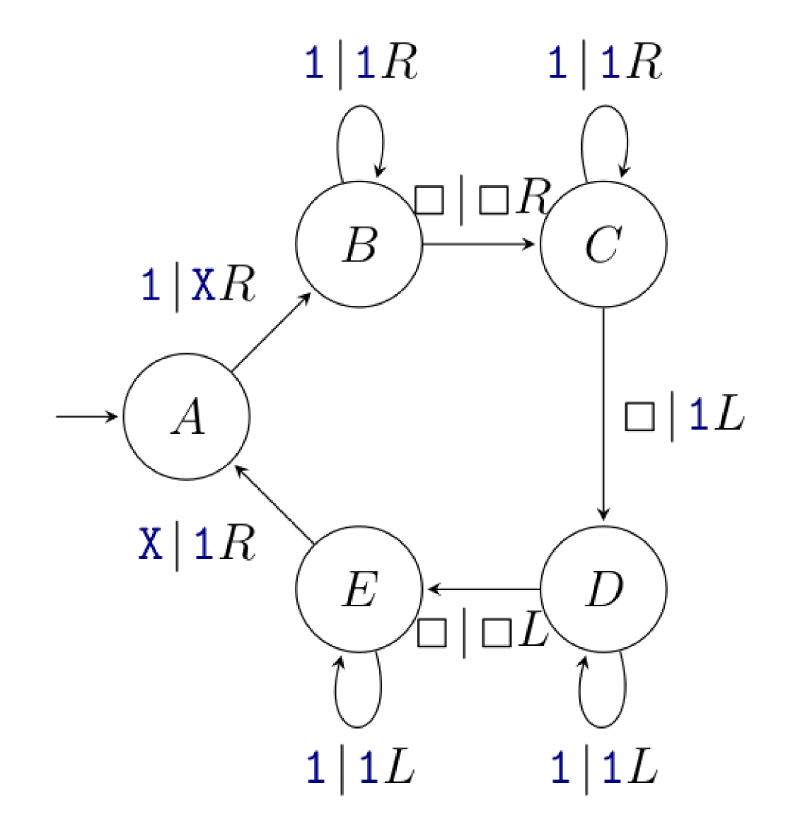
\includegraphics[height=5cm]{copyTM.png}
  \end{figure}
  \begin{center}
    \begin{tabular}{cccccc}
      \toprule
      & A       & B      & C       & D       & E \\
      \midrule
      $\square$&         & C,$\square$,R & D,1,L & E,$\square$,L  &  \\
      1         & B,X,R & B,1,R& C,1,R & D,1,L & E,1,L \\
      X         &         &        &         &         & A,1,R \\
      \bottomrule
    \end{tabular}
  \end{center}
\end{frame}
\begin{frame}[plain]
  \frametitle{Aufgabe}
  Welche Sprache akzeptiert diese TM?
  \begin{figure}
    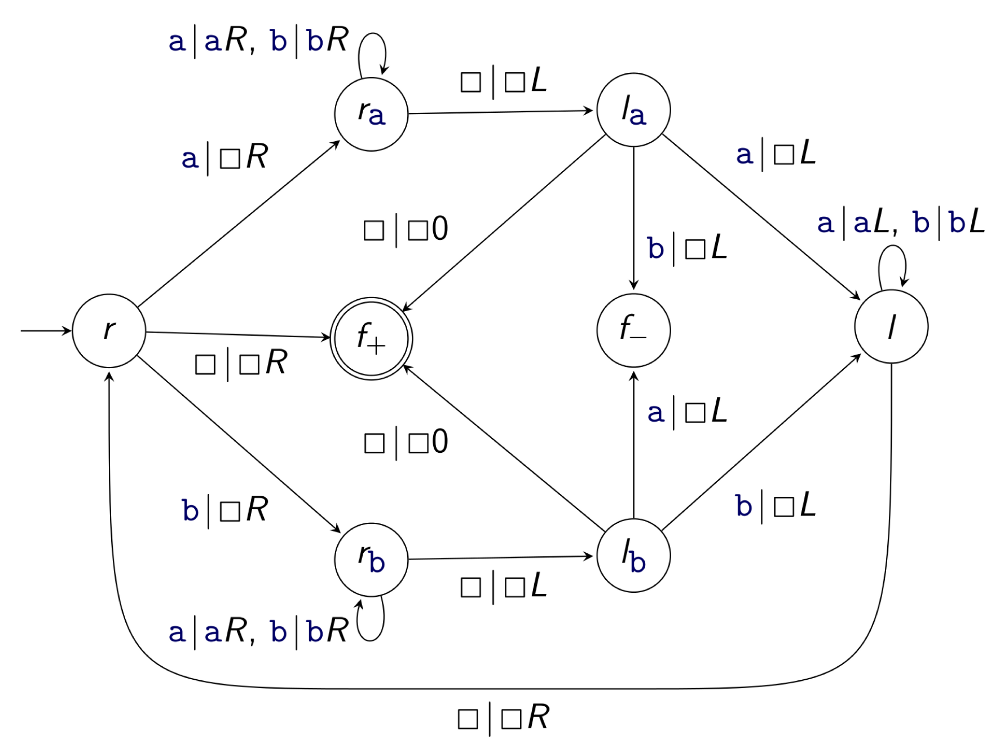
\includegraphics[height=7cm]{palindromTM.png}
  \end{figure}
\end{frame}
\begin{frame}
  \frametitle{Aufgabe}
  \begin{center}
    \begin{tabular}{cccccc}
      \toprule
      & r & $c_0$ & $c_1$ & h \\
      \midrule
      0 & r,0,R   & $c_0$,0,L & $c_0$,1,L \\
      1 & r,1,R   & $c_0$,1,L & $c_1$,0,L \\
      $\square$  & $c_1$,$\square$, L & h,$\square$ ,R   & $c_0$,1,L & \hphantom{C,1,L} \\
      \bottomrule
    \end{tabular}
  \end{center}
  \begin{enumerate}
    \item Zeichnet die Turingmachine.
    \item Was berechnet die Turingmaschine?\\
    \ans{2}{Sie erhöht das Wort auf dem Band um 1, wenn man es als Binärzahl interpretiert.}
  \end{enumerate}
\end{frame}

\section{Entscheidbarkeits-Theorie}
\begin{frame}
	\frametitle{Entscheidbarkeit}
	\begin{exampleblock}{}
    Eine Sprache heißt $\dots$
		\begin{description}
			\item[aufzählbar:] es gibt eine Turingmaschine, die die Sprache akzeptiert
			\item [entscheidbar:] es gibt eine Turingmaschine, die \emph{immer hält} und die Sprache akzeptiert
		\end{description}
	\end{exampleblock}
	\begin{alertblock}{Achtung}
		Entscheidbarkeit ist stärkere Forderung
	\end{alertblock}
\end{frame}

\section{Komplexitätstheorie}
\subsection*{}
\begin{frame}
	\frametitle{Zeitkomplexität}
	\begin{block}{Zwei Maße für den Zeitbedarf}
		\begin{itemize}
			\item $\text{time}_T(w)=$ das $t$ mit $\Delta_t(c_0(w))=\Delta_*(c_0(w))$
			\item $\text{Time}_T(w)=\max\{\text{time}_T(w)|w\in A^n\}$
		\end{itemize}
	\end{block}
\end{frame}
\begin{frame}
	\frametitle{Raumkomplexität}
	\begin{block}{Zwei Maße für den Platzbedarf}
		\begin{itemize}
			\item $\text{space}_T(w)=$ die Anzahl der benötigten Felder (Felder die vom Schreiblesekopf "`besucht"' werden)
			\item $\text{Space}_T(w)=\max\{\text{space}_T(w)|w\in A^n\}$
		\end{itemize}
	\end{block}
\end{frame}
\begin{frame}
	\frametitle{Zeit- und Raumkomplexität}
	\begin{block}{Zusammenhang}
		Eine TM, die time($w$) Schritte macht, kann auch nur höchstens $1+\text{time}(w)$ Felder besuchen.\\
		Also gilt:
		$$\text{space}(w)\leq \max(|w|, 1+\text{time}(w))$$
	\end{block}
\end{frame}
\begin{frame}
  \frametitle{P und PSPACE}
  P und PSPACE sind Mengen von \emph{Sprachen} für die das Problem: $w \in L$ gelöst werden soll.
	\begin{description}
		\item[P:] Sprachen die von Turingmaschinen entschieden werden können, deren Zeitkomplexität polynomiell ist.
		\item[PSPACE:] Sprachen die von Turingmaschinen entschieden werden können, deren Raumkomplexität polynomiell ist.
	\end{description}
	\begin{block}{P $\subseteq$ PSPACE}
		Leicht zu sehen durch den erwähnten Zusammenhang zwischen Raum- und Zeitkomplexität.
	\end{block}
	\pause
	\begin{alertblock}{PSPACE $\subseteq$ P ?}
		Ein ungelöstes Problem der Informatik
	\end{alertblock}
\end{frame}


